\documentclass[tikz,border=8pt]{standalone}
% Shared look for every TikZ diagram. Load with \input{../../tools/tikz-style.tex}
\usepackage[sfdefault]{roboto}
\usetikzlibrary{arrows.meta, positioning, shapes.geometric, calc, fit, backgrounds}
\definecolor{cblue}{HTML}{4C78A8}
\definecolor{corange}{HTML}{F58518}
\definecolor{cgreen}{HTML}{54A24B}
\definecolor{cred}{HTML}{E45756}
\definecolor{cpurple}{HTML}{B279A2}
\definecolor{cgrey}{HTML}{6B6B6B}
\tikzset{
  every picture/.style={font=\sffamily, line width=1.2pt},
  box/.style={draw=#1, fill=#1!12, rounded corners=4pt, align=center, inner sep=7pt, minimum height=1.1cm},
  box/.default=cgrey,
  arrow/.style={-{Stealth[length=3mm]}, draw=cgrey, line width=1.4pt},
  title/.style={font=\sffamily\bfseries\Large},
  note/.style={font=\sffamily\small, text=cgrey, align=center},
}
\AtBeginDocument{\hyphenpenalty=10000 \exhyphenpenalty=10000}

% Autoware Universe trajectory follower, read from the code (2026-10-12): autoware_planning_msgs/TrajectoryPoint has
% time_from_start, pose, longitudinal_velocity_mps; controller_node.cpp picks the lateral controller (mpc or
% pure_pursuit) and the longitudinal one (pid); trajectory_follower_node.param.yaml: trajectory_reference_mode "spatial"
% (default) or "temporal", ctrl_period 0.03 s.
\begin{document}
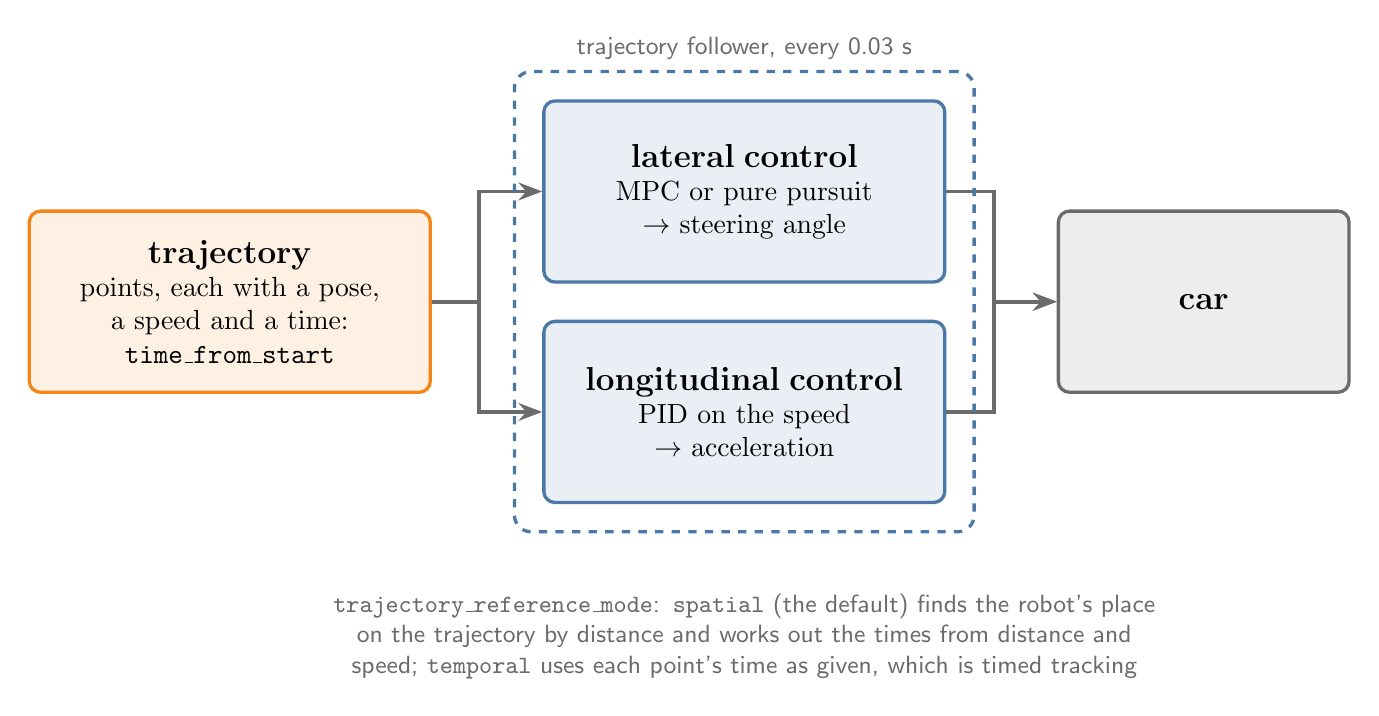
\begin{tikzpicture}[node distance=0.6cm,
  st/.style={box=#1, font=\normalsize, text width=4.6cm, minimum height=2.3cm}]
  \node[st=corange] (traj) {{\large\textbf{trajectory}}\\ points, each with a pose,\\ a speed and a time:\\ \texttt{time\_from\_start}};
  \node[st=cblue, right=1.4cm of traj, yshift=1.4cm] (lat) {{\large\textbf{lateral control}}\\ MPC or pure pursuit\\ $\rightarrow$ steering angle};
  \node[st=cblue, right=1.4cm of traj, yshift=-1.4cm] (lon) {{\large\textbf{longitudinal control}}\\ PID on the speed\\ $\rightarrow$ acceleration};
  \node[st=cgrey, right=1.4cm of lat, yshift=-1.4cm, text width=3.2cm] (car) {{\large\textbf{car}}};
  \draw[arrow] (traj.east) -- ++(0.6,0) |- (lat.west);
  \draw[arrow] (traj.east) -- ++(0.6,0) |- (lon.west);
  \draw[arrow] (lat.east) -- ++(0.6,0) |- (car.west);
  \draw[arrow] (lon.east) -- ++(0.6,0) |- (car.west);
  \node[draw=cblue, dashed, rounded corners=6pt, inner sep=10pt, fit=(lat) (lon), label={[note]above:trajectory follower, every 0.03 s}] {};
  \node[note, anchor=north, text width=15cm] at ([yshift=-1.0cm]lon.south) {\texttt{trajectory\_reference\_mode}: \texttt{spatial} (the default) finds the robot's place on the trajectory by distance and works out the times from distance and speed; \texttt{temporal} uses each point's time as given, which is timed tracking};
\end{tikzpicture}
\end{document}
